\chapter{Optimisation}
\label{ch-opt}

\section{Méthode}

Les actions sont appliquées une à la fois. Après chaque action, les prédictions sont recalculées et notre script mesure la couverture par zone sur les rasters exportés, de la même façon pour toutes les actions. L'action est gardée si elle améliore les objectifs sans dégrader le reste, et annulée sinon. Les mesures avant et après sont ainsi comparables d'une action à l'autre. Cette boucle reprend celle du cours : prédictions de couverture et d'interférence, ajustement, puis densification~\cite{afif2026cours}.

\section{Diagnostic}

Après les deux premières actions, il reste \SI{13,0}{\kilo\metre\squared} de trous ruraux en outdoor. Pour atteindre \SI{95}{\percent} des \SI{76,95}{\kilo\metre\squared} ruraux, au plus \SI{3,85}{\kilo\metre\squared} peuvent rester découverts : il faut regagner environ \SI{9}{\kilo\metre\squared}.

\begin{figure}[H]
\centering
\begin{minipage}[c]{0.44\textwidth}\centering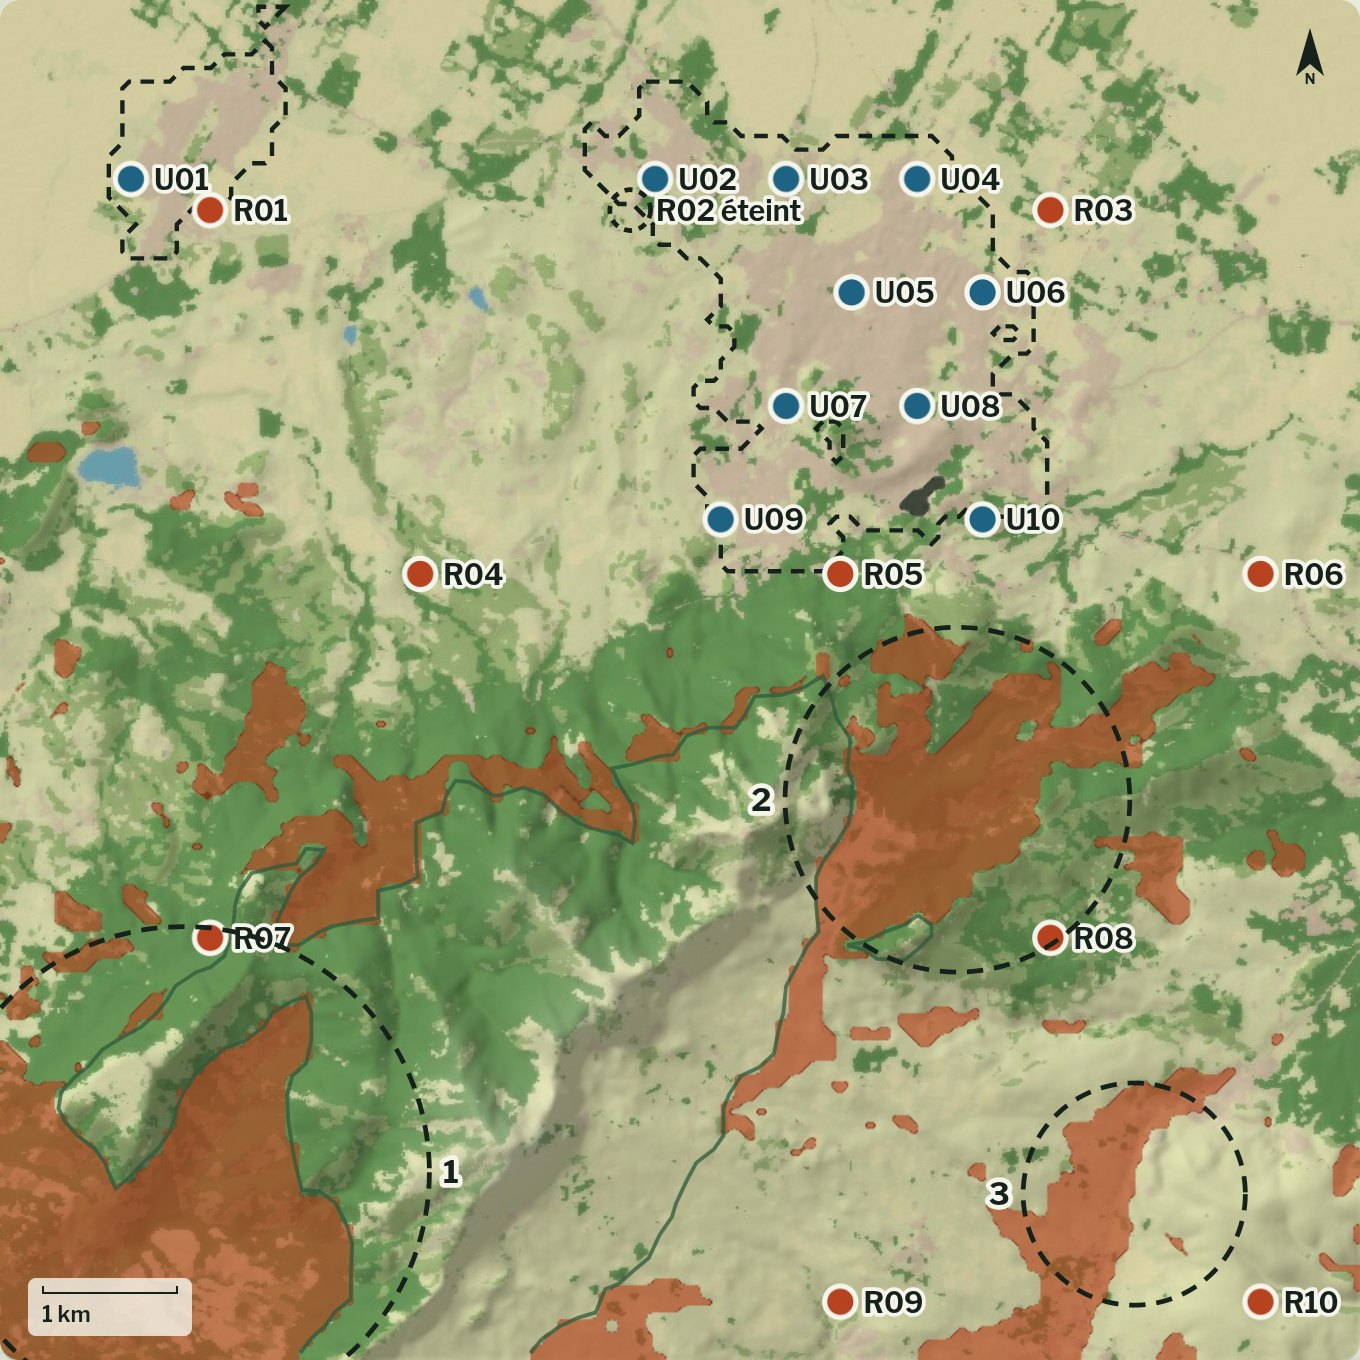
\includegraphics[width=\textwidth]{diagnostic.jpg}\end{minipage}\hfill
\begin{minipage}[c]{0.52\textwidth}
\captionof{table}{Trous ruraux (raster d'Atoll).}
\label{tab-trous}
\footnotesize
\begin{tabular}{@{}lrr@{}}
\toprule
\thead{Trou} & \thead{Surface} & \thead{Habitants} \\
\midrule
1 · coin sud-ouest & \SI{4,84}{\kilo\metre\squared} & 128 \\
2 · pied est de la crête & \SI{3,25}{\kilo\metre\squared} & 144 \\
3 · sud-est & \SI{1,81}{\kilo\metre\squared} & 198 \\
poches ouest et nord-ouest & \SI{2,09}{\kilo\metre\squared} & 52 \\
\midrule
total, avec les pixels isolés & \SI{13,0}{\kilo\metre\squared} & \\
\bottomrule
\end{tabular}
\end{minipage}
\captionof{figure}{Trous ruraux avant les actions de couverture.}
\label{fig-diag}
\end{figure}

En ville, la couverture est atteinte ; le problème est l'interférence (\cref{sec-cinr}), due à trop de recouvrement et à un tilt trop faible. Les actions 1, 2 et 7 visent la ville, les actions 3 à 6 la campagne.

\section{Action 1 : tilt urbain de 4° à 6°}

Le diagramme vertical de l'antenne, relevé dans Atoll, a une ouverture d'environ \ang{6,3} à \SI{-3}{\deci\bel} et n'est atténué que de \SI{4,1}{\deci\bel} à l'horizon. Avec un tilt de \ang{4}, le bord supérieur du lobe (\ang{3,4} au-dessus de l'axe) n'est incliné que de \ang{0,6} et touche le sol à $30 / \tan 0{,}6^\circ \approx \SI{2,9}{\kilo\metre}$, cinq fois le rayon de la cellule : chaque secteur arrose ses voisins. Le tilt qui place ce bord au bord de la cellule vaut
\begin{equation}
  \arctan\!\left(\frac{30}{640}\right) + 3{,}4^\circ \approx 2{,}7^\circ + 3{,}4^\circ \approx 6{,}1^\circ .
\end{equation}
Nous avons ajouté \ang{2} de tilt mécanique aux \ang{4} électriques des secteurs urbains. La \cref{fig-tilt} montre l'effet : avec \ang{6}, le bord du lobe touche le sol à \SI{0,66}{\kilo\metre}, au bord de la cellule.

\begin{figure}[H]
\centering
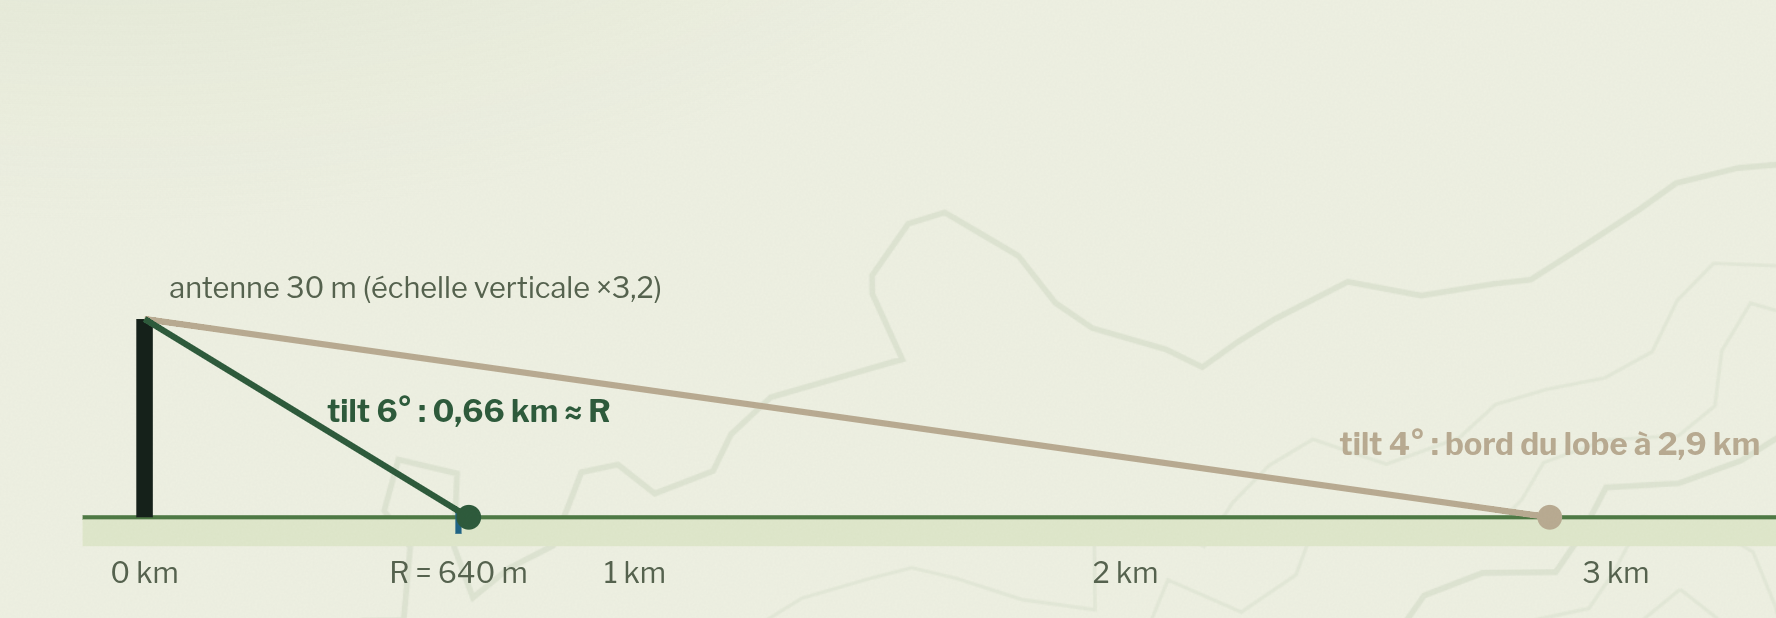
\includegraphics[width=0.8\textwidth]{tilt.png}
\caption{Géométrie du tilt urbain (échelle verticale × 3,2).}
\label{fig-tilt}
\end{figure}

\begin{table}[H]
\centering
\caption{Action 1 : tilt urbain de \ang{4} à \ang{6}.}
\label{tab-a1}
\begin{tabular}{@{}lccc@{}}
\toprule
\thead{Indicateur} & \thead{Avant} & \thead{Après} & \thead{Évolution} \\
\midrule
Surface à 4 serveurs ou plus & \SI{2,39}{\kilo\metre\squared} & \SI{1,45}{\kilo\metre\squared} & $-\SI{39}{\percent}$ \\
Surface C/(I+N) $\geq \SI{-1}{\deci\bel}$ & \SI{13,1}{\kilo\metre\squared} & \SI{14,6}{\kilo\metre\squared} & $+\SI{11}{\percent}$ \\
Couverture urbaine indoor & \SI{99,5}{\percent} & \SI{99,4}{\percent} & $-0{,}1$ pt \\
Couverture rurale outdoor & \SI{83,4}{\percent} & \SI{83,2}{\percent} & sites ruraux inchangés \\
\bottomrule
\end{tabular}
\end{table}

\begin{verdict}
Action \gardee{} (mesures à charge \SI{100}{\percent}) : le recouvrement à quatre serveurs baisse de \SI{39}{\percent} et la surface de bonne qualité augmente de \SI{11}{\percent}, pour une perte de couverture urbaine négligeable.
\end{verdict}

\section{Action 2 : désactivation du site R02}

R02, site rural de la grille nominale, se trouve à \SI{300}{\metre} du site urbain U02. Il a été désactivé plutôt que supprimé, car Atoll efface toutes les simulations qui utilisent un site supprimé. Les mesures du \cref{tab-a2} utilisent les charges simulées à \num{1000} utilisateurs.

\begin{table}[H]
\centering
\caption{Action 2 : désactivation de R02.}
\label{tab-a2}
\begin{tabular}{@{}lccc@{}}
\toprule
\thead{Indicateur} & \thead{Avant} & \thead{Après} & \thead{Évolution} \\
\midrule
Couverture urbaine indoor & \SI{99,4}{\percent} & \SI{99,4}{\percent} & 0 \\
Couverture rurale outdoor & \SI{83,2}{\percent} & \SI{83,1}{\percent} & $-0{,}1$ pt \\
Surface à 2 serveurs ou plus & \SI{24,37}{\kilo\metre\squared} & \SI{23,10}{\kilo\metre\squared} & $-\SI{5}{\percent}$ \\
Surface C/(I+N) $\geq \SI{-1}{\deci\bel}$ & \SI{36,13}{\kilo\metre\squared} & \SI{36,82}{\kilo\metre\squared} & $+\SI{2}{\percent}$ \\
Nombre de sites & 20 & 19 & $-1$ \\
\bottomrule
\end{tabular}
\end{table}

\begin{verdict}
Action \gardee{} : le gain radio est faible, mais un site entier est économisé (pylône, équipements, énergie, loyer) sans perte de couverture. R01, également proche d'un site urbain, a été conservé : la simulation montre que sa cellule R01\_1 est la plus chargée du réseau, car elle sert le village du nord-ouest.
\end{verdict}

\section{Actions 3 et 3b : déplacer ou réorienter R07, rejetées}

R07 est placé sur le flanc du massif, à \SI{503}{\metre}. Première idée (action 3) : le déplacer au centre du trou sud-ouest, à \SI{391}{\metre}. Seconde idée (action 3b) : le laisser en place et tourner ses secteurs vers le coin (azimuts \ang{30}, \ang{190}, \ang{290}).

\begin{table}[H]
\centering
\caption{Actions 3 et 3b, mesurées puis annulées.}
\label{tab-a3}
\small\setlength{\tabcolsep}{5pt}
\begin{tabular}{@{}lccl@{}}
\toprule
\thead{Action} & \thead{Rural\\outdoor (surface)} & \thead{Rural\\(population)} & \thead{Verdict} \\
\midrule
Avant (R02 désactivé) & \SI{83,1}{\percent} & \SI{95,2}{\percent} & \\
3 · R07 déplacé dans le coin sud-ouest & \SI{82,7}{\percent} & \SI{94,7}{\percent} & \rejetee \\
3b · R07 réorienté (\ang{30}/\ang{190}/\ang{290}) & \SI{82,4}{\percent} & \SI{95,1}{\percent} & \rejetee \\
\bottomrule
\end{tabular}
\end{table}

Déplacé, R07 couvre le coin mais ne voit plus la plaine ouest qu'il servait depuis sa hauteur. Réorienté, il ne gagne que \SI{0,01}{\kilo\metre\squared} dans le coin (comparaison pixel à pixel). Le profil du terrain explique ces deux échecs (\cref{fig-profil}). R07 est à \SI{503}{\metre}, plus \SI{30}{\metre} de mât, et le coin sud-ouest à \SI{389}{\metre}, à \SI{2,4}{\kilo\metre} ; entre les deux, la crête monte à \SI{807}{\metre} et coupe la ligne de vue. Changer l'azimut ne sert à rien : seul un site placé dans le coin peut servir cette zone d'ombre.

\begin{figure}[H]
\centering
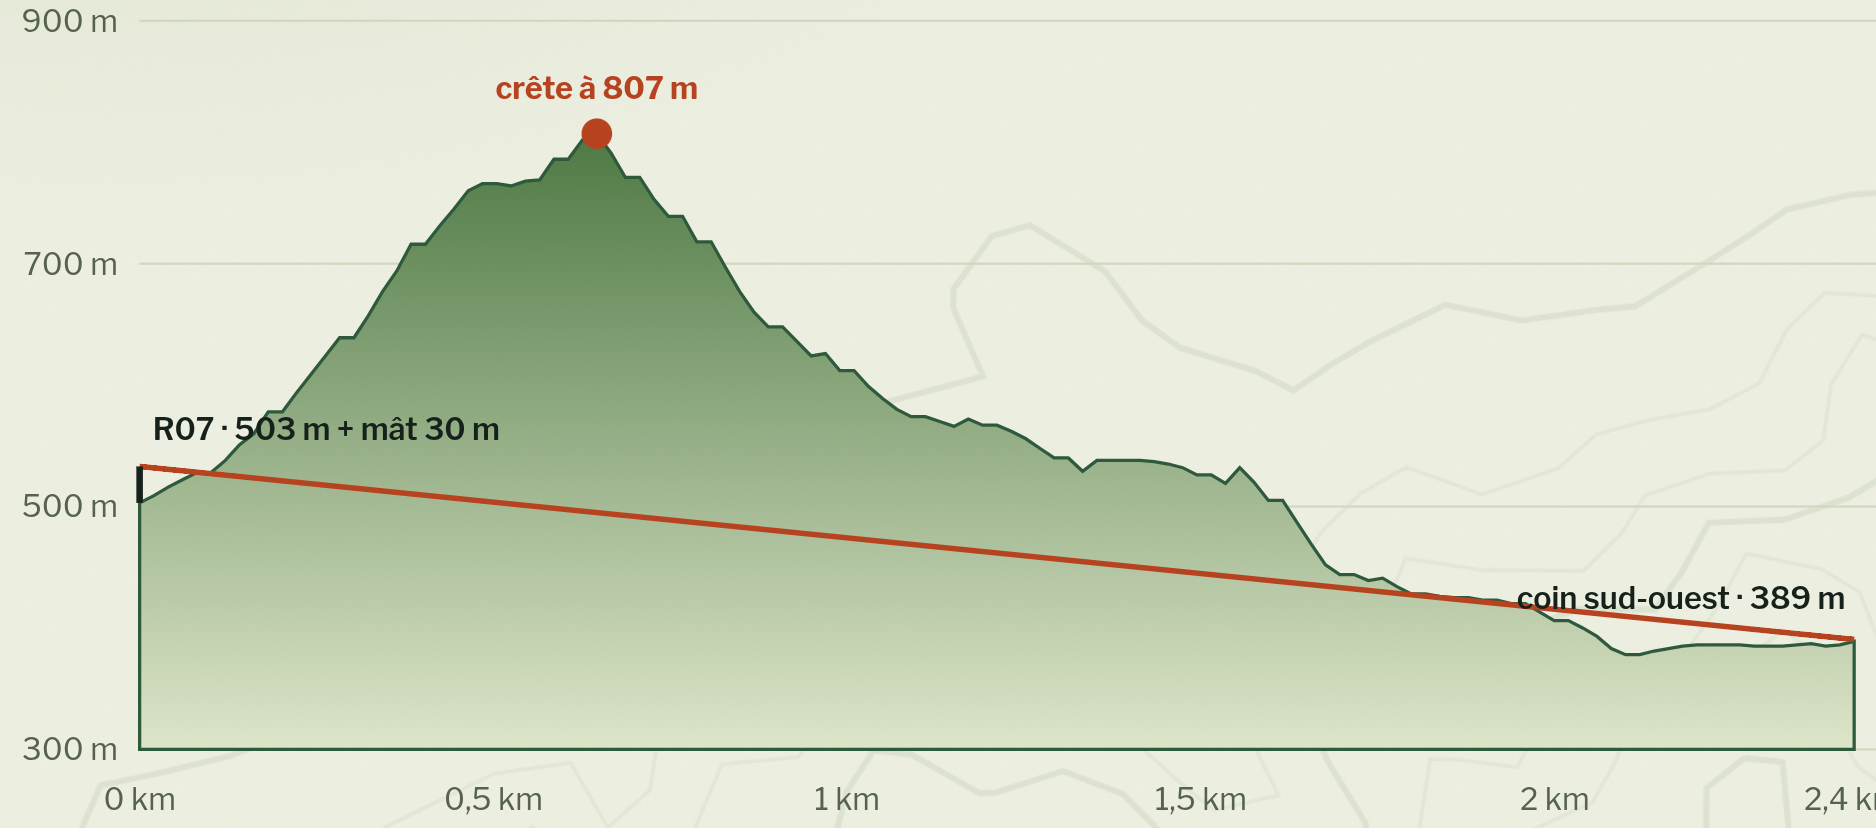
\includegraphics[width=0.85\textwidth]{profil-r07.png}
\caption{Profil du terrain entre R07 et le coin sud-ouest.}
\label{fig-profil}
\end{figure}

\section{Actions 4 et 5 : deux sites là où le relief l'exige}

Le budget de R02 est déplacé là où la couverture manque : un site R11 est créé au centre du trou sud-ouest (X = \SI{597240}{\metre}, Y = \SI{4023060}{\metre}, \SI{391}{\metre}), puis un site R12 au centre du trou du pied est (X = \SI{603230}{\metre}, Y = \SI{4026200}{\metre}).

\begin{table}[H]
\centering
\caption{Actions 4 et 5 : ajout des sites R11 et R12.}
\label{tab-a45}
\small\setlength{\tabcolsep}{5pt}
\begin{tabular}{@{}lccccl@{}}
\toprule
\thead{Étape} & \thead{Rural\\(surface)} & \thead{Rural\\(population)} & \thead{Urbain\\indoor} & \thead{Sites} & \thead{Verdict} \\
\midrule
Avant & \SI{83,1}{\percent} & \SI{95,2}{\percent} & \SI{99,4}{\percent} & 19 & \\
4 · + R11 (sud-ouest) & \SI{87,1}{\percent} & \SI{95,8}{\percent} & \SI{99,4}{\percent} & 20 & \gardee \\
5 · + R12 (pied est) & \SI{90,3}{\percent} & \SI{96,6}{\percent} & \SI{99,4}{\percent} & 21 & \gardee \\
\bottomrule
\end{tabular}
\end{table}

\begin{figure}[H]
\centering
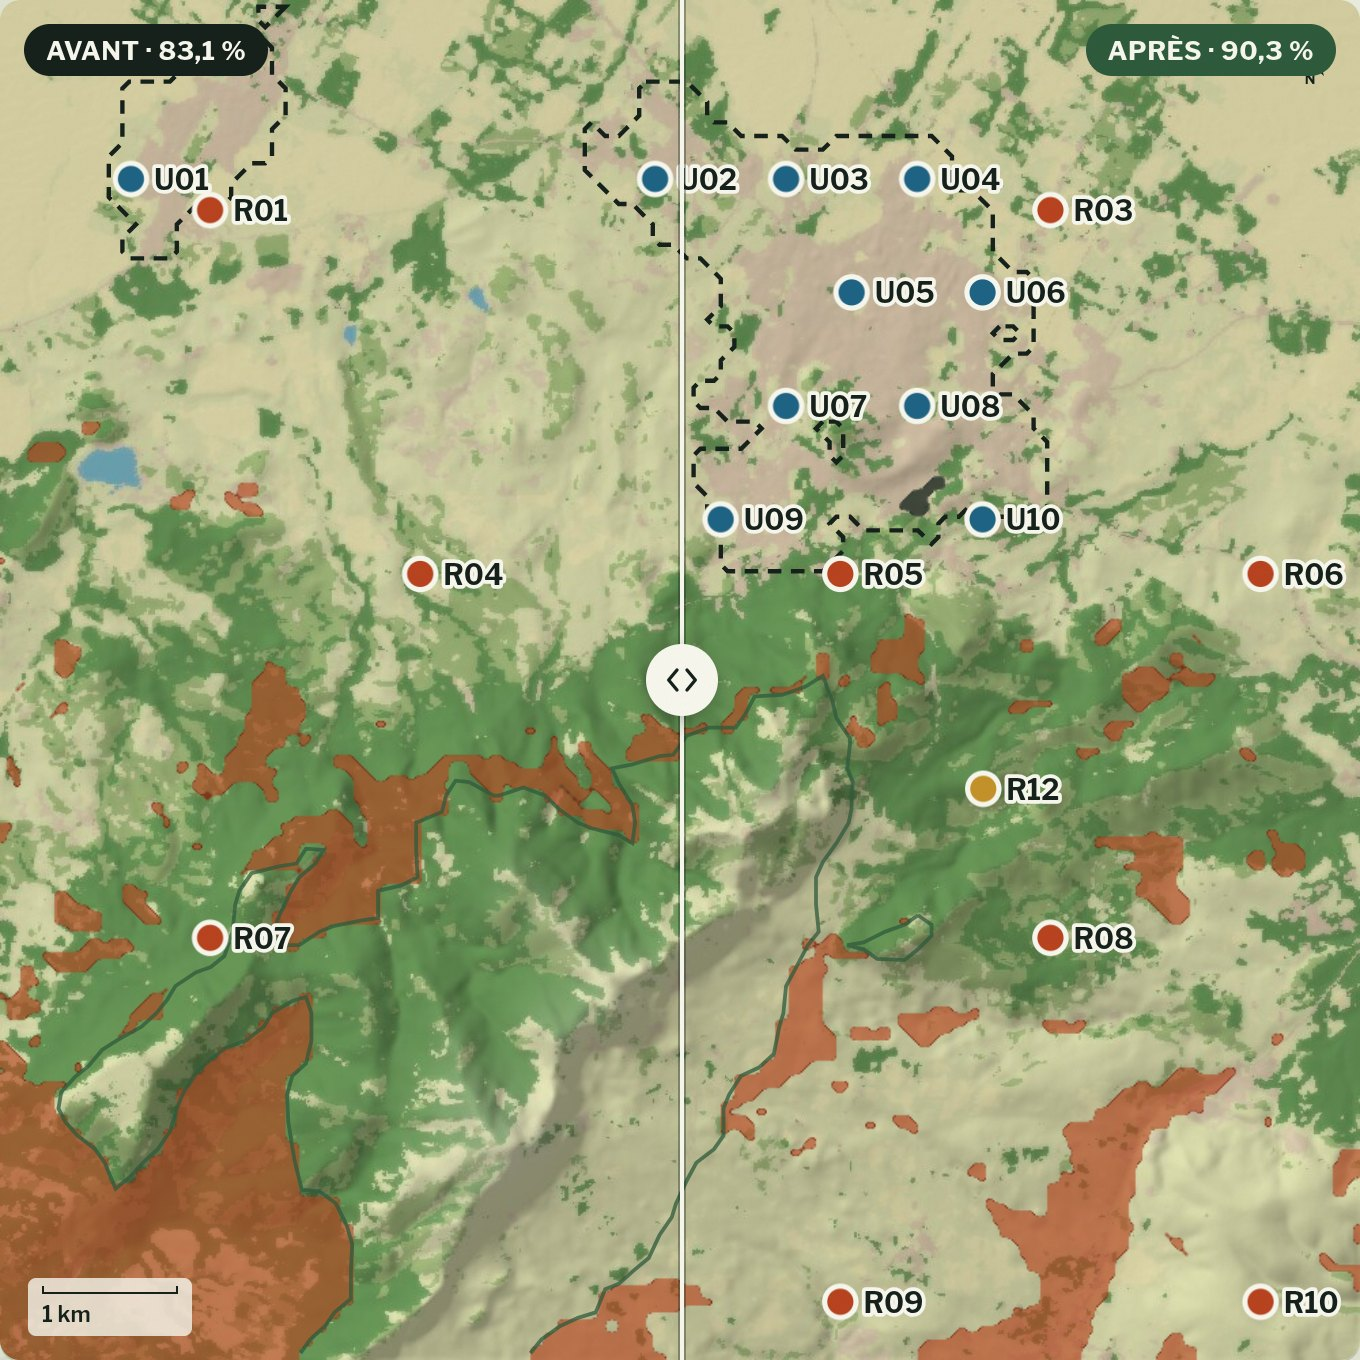
\includegraphics[width=0.58\textwidth]{r11-r12.jpg}
\caption{Couverture avant et après l'ajout de R11 et R12.}
\label{fig-r11r12}
\end{figure}

Sur la \cref{fig-r11r12}, la carte de gauche est le réseau sans R02, celle de droite le réseau avec R11 et R12 (en or) : les deux grands trous ruraux sont comblés.

Le réseau compte alors 21 sites, le nombre prévu par l'Étape 1, mais pas aux mêmes endroits. Nous n'ajoutons pas d'autre site. Il reste 4,7 points à gagner : le meilleur site suivant (au sud-est) apporterait environ 2,3 points, et il en faudrait encore environ trois pour atteindre \SI{95}{\percent} en surface, pour quelque 300 habitants dispersés, alors que \SI{96,6}{\percent} de la population rurale est déjà couverte. La suite est confiée au réglage automatique des antennes.

\section{Action 6 : planification automatique (ACP)}

Le module ACP (\emph{Automatic Cell Planning}) d'Atoll cherche la combinaison de réglages d'antennes qui maximise des objectifs de couverture. Nous lui avons donné nos objectifs : RSRP $\geq \SI{-120}{\dBm}$ sur \SI{95}{\percent} de la zone (son seuil par défaut était \SI{-105}{\dBm}) et RSRQ $\geq \SI{-15}{\deci\bel}$ sur \SI{85}{\percent}. Les réglages autorisés étaient le tilt électrique (\ang{0} à \ang{10}), l'azimut (± \ang{20}) et le tilt mécanique (\ang{0} à \ang{5}) ; la sélection de sites a été désactivée, car les sites sont décidés par nos actions mesurées. Le calcul (380 itérations) converge après environ 90 itérations.

\begin{figure}[H]
\centering
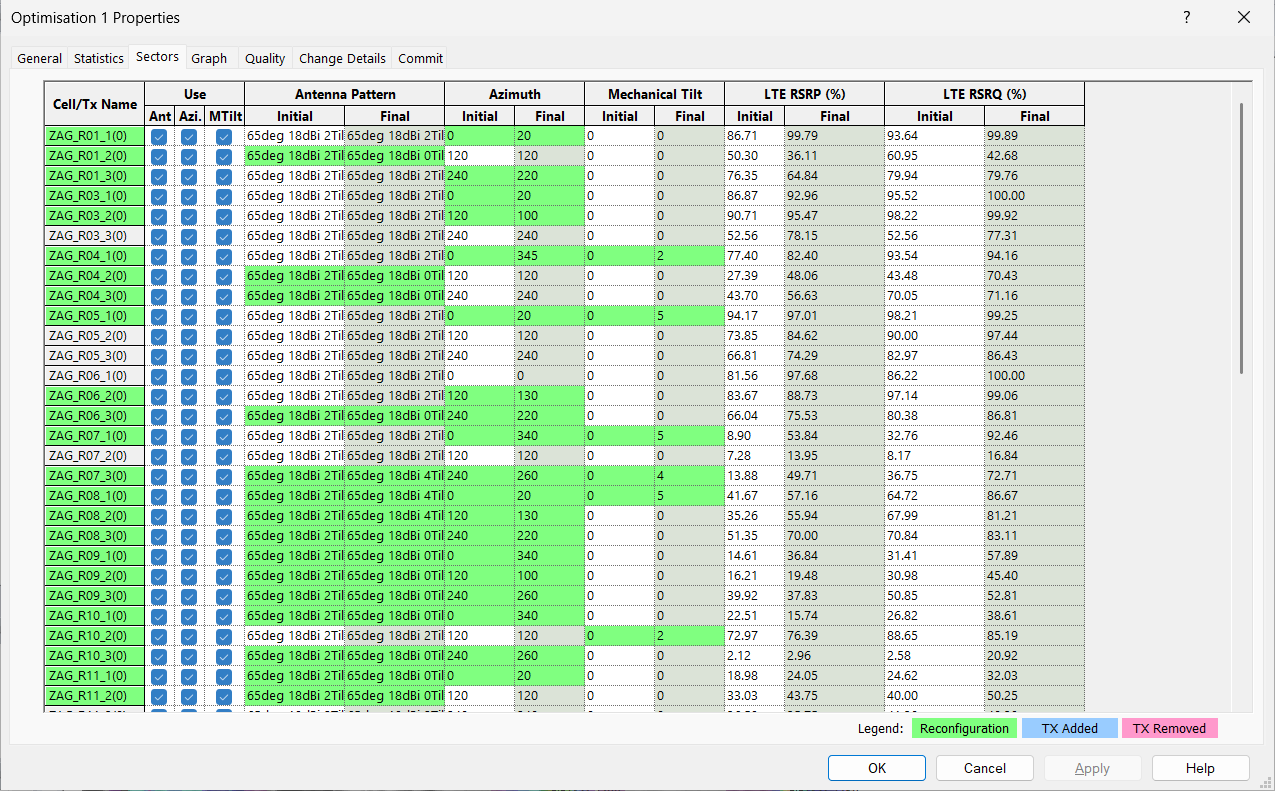
\includegraphics[width=0.75\textwidth]{acp_secteurs.png}
\caption{Changements proposés par l'ACP, secteur par secteur.}
\label{fig-acp}
\end{figure}

La \cref{fig-acp} détaille les propositions. L'ACP propose une soixantaine de changements, surtout sur les secteurs ruraux : beaucoup de tilts électriques ramenés de \ang{2} à \ang{0} pour porter plus loin, quelques secteurs basculés de \ang{2} à \ang{4}, des azimuts tournés jusqu'à \ang{20} et un tilt mécanique sur certains secteurs tournés vers la ville. Il relève aussi trois secteurs urbains de bordure orientés vers la campagne (U01\_3, U02\_3, U09\_3). Les premiers changements apportent l'essentiel du gain.

L'ACP évalue ses objectifs sur toute la zone de calcul d'Atoll (\SI{240}{\kilo\metre\squared}, en grande partie hors de nos cartes et loin des sites), d'où une couverture de départ de \SI{21,7}{\percent} selon sa propre mesure. Nous n'utilisons donc que son gain \emph{relatif} (+4,3 points) et vérifions chaque proposition avec nos propres prédictions :

\begin{table}[H]
\centering
\caption{Action 6 : réglages de l'ACP.}
\label{tab-acp}
\begin{tabular}{@{}lccc@{}}
\toprule
\thead{Indicateur} & \thead{Avant ACP} & \thead{Après ACP} & \thead{Évolution} \\
\midrule
Couverture rurale outdoor (surface) & \SI{90,3}{\percent} & \textbf{\SI{94,3}{\percent}} & +4,0 pts \\
Couverture rurale outdoor (population) & \SI{96,6}{\percent} & \SI{97,9}{\percent} & +1,3 pt \\
Couverture urbaine indoor & \SI{99,4}{\percent} & \SI{99,7}{\percent} & +0,3 pt \\
\bottomrule
\end{tabular}
\end{table}

\begin{verdict}
Action \gardee{} : le gain mesuré sur notre zone (+4,0 points) correspond au gain annoncé par l'ACP sur la sienne (+4,3 points). Il reste 0,7 point (environ \SI{0,5}{\kilo\metre\squared}) pour atteindre \SI{95}{\percent}, moins que l'incertitude du modèle.
\end{verdict}

\section{Action 7 : tilt urbain à 8°, rejetée}

Pour réduire encore l'interférence urbaine, les secteurs urbains ont été basculés à \ang{8}. Le DL en ville gagne 1,2 point (de \SI{79,4}{\percent} à \SI{80,6}{\percent} de la surface à \SI{1}{\Mbps}), un écart dans le bruit du modèle, tandis que la campagne perd 0,1 point de couverture et 0,6 point de DL. L'action est \rejetee{} : le tilt de \ang{6} est déjà proche de l'optimum géométrique de \ang{6,1}.

\section{Action 8 : relations de voisinage (ANR)}

Le module ANR (\emph{Automatic Neighbour Relations}) construit les listes de voisins utilisées pour le handover. Il a été lancé avec une distance maximale de \SI{10}{\kilo\metre}, au plus 16 voisins par cellule, une marge de handover de \SI{0}{} à \SI{5}{\deci\bel} (la marge de notre carte de recouvrement) et des relations symétriques. Il attribue en général 3 à 6 voisins par cellule. L'ANR ne change pas les cartes radio ; il permet le handover entre les cellules qui se recouvrent, utile pour les utilisateurs mobiles. Après le tilt de \ang{6}, les cellules urbaines n'ont pas beaucoup plus de voisins que les cellules rurales, signe que le recouvrement a été contenu.

\section{Le réseau final}
\label{sec-final}

Le réseau final compte 21 sites : le réseau initial, sans R02, avec R11 et R12, le tilt urbain de \ang{6} et les réglages de l'ACP. Une nouvelle simulation à \num{1000} utilisateurs, avec la même graine, a fourni les charges finales, puis toutes les prédictions ont été recalculées.

\begin{figure}[H]
\centering
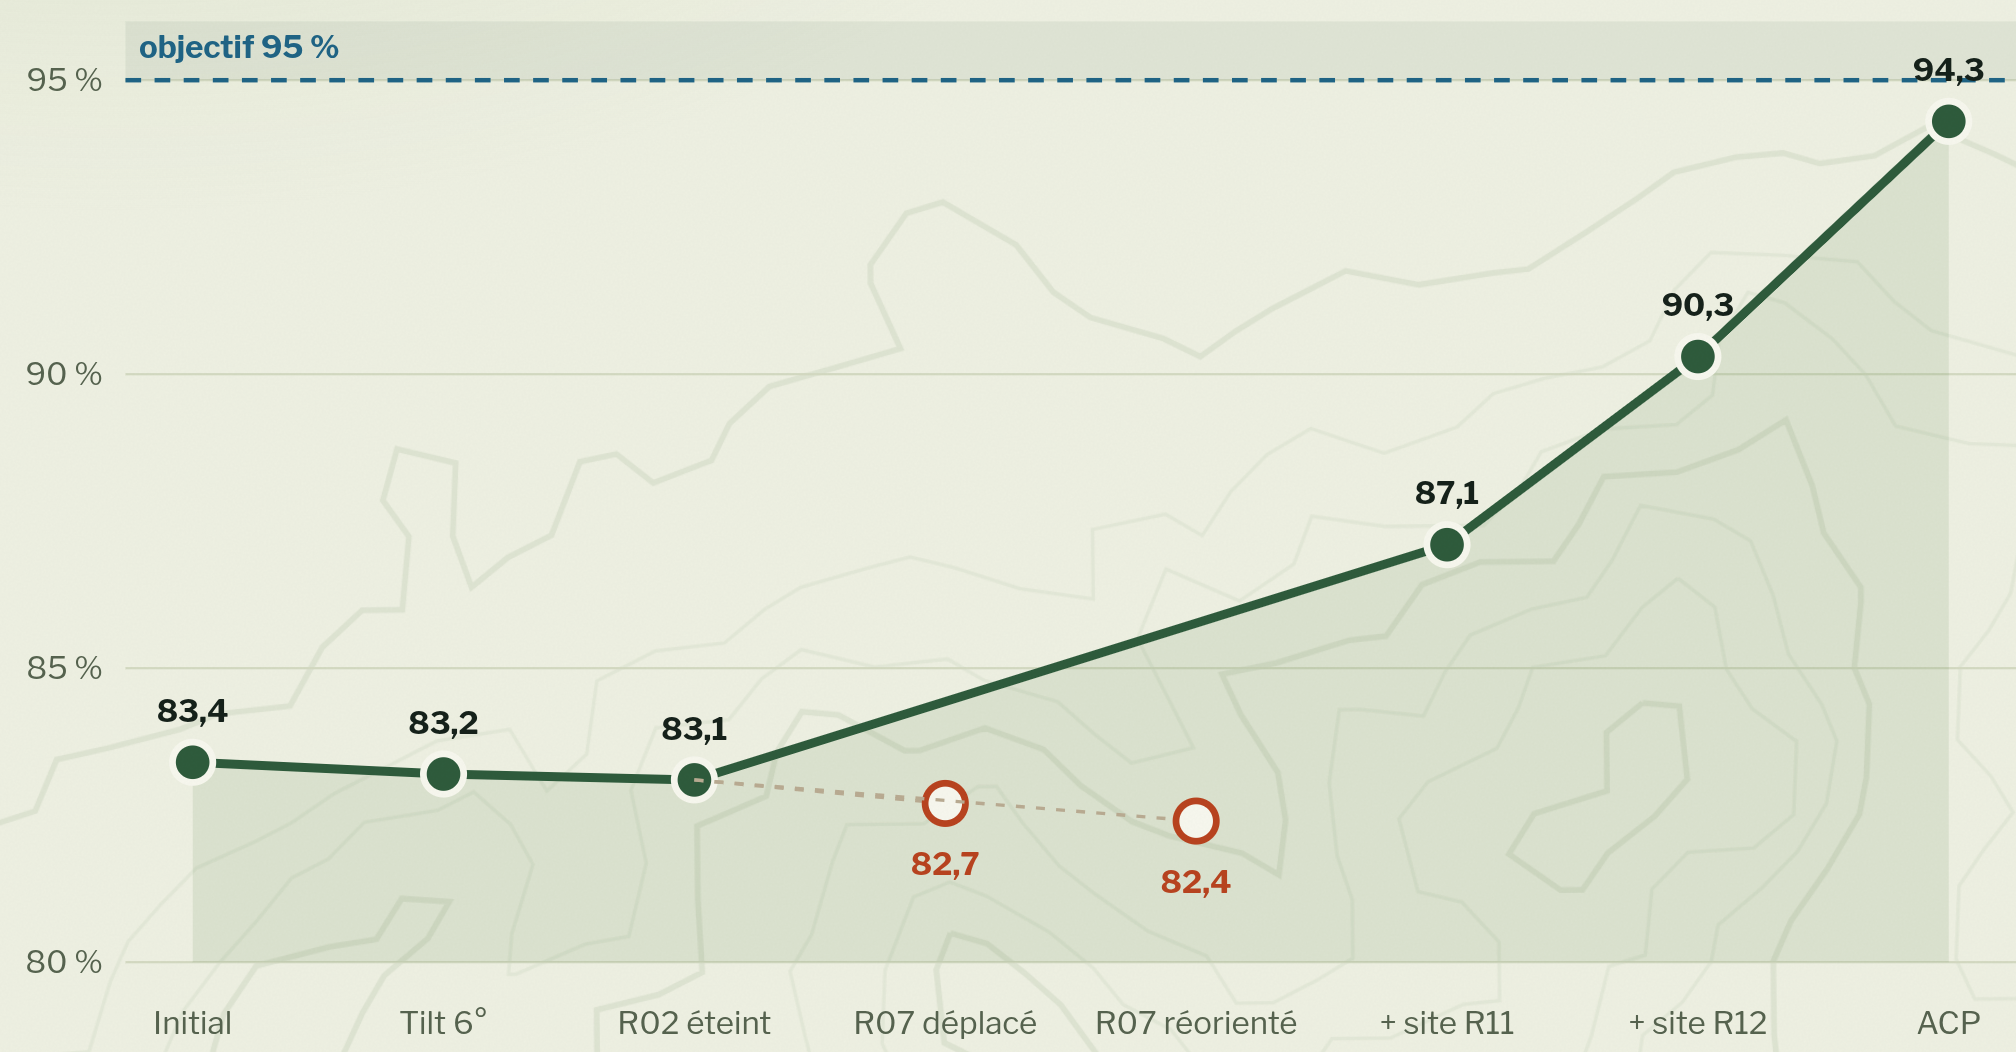
\includegraphics[width=0.9\textwidth]{progression.png}
\caption{Couverture rurale outdoor après chaque action.}
\label{fig-progression}
\end{figure}

Sur la \cref{fig-progression}, les cercles creux sont les actions rejetées, mesurées puis annulées ; la ligne pointillée est l'objectif de \SI{95}{\percent}. Sur la \cref{fig-ombre-final}, R11 et R12 (en or) sont posés à l'intérieur de l'ombre de la crête.

\begin{figure}[H]
\centering
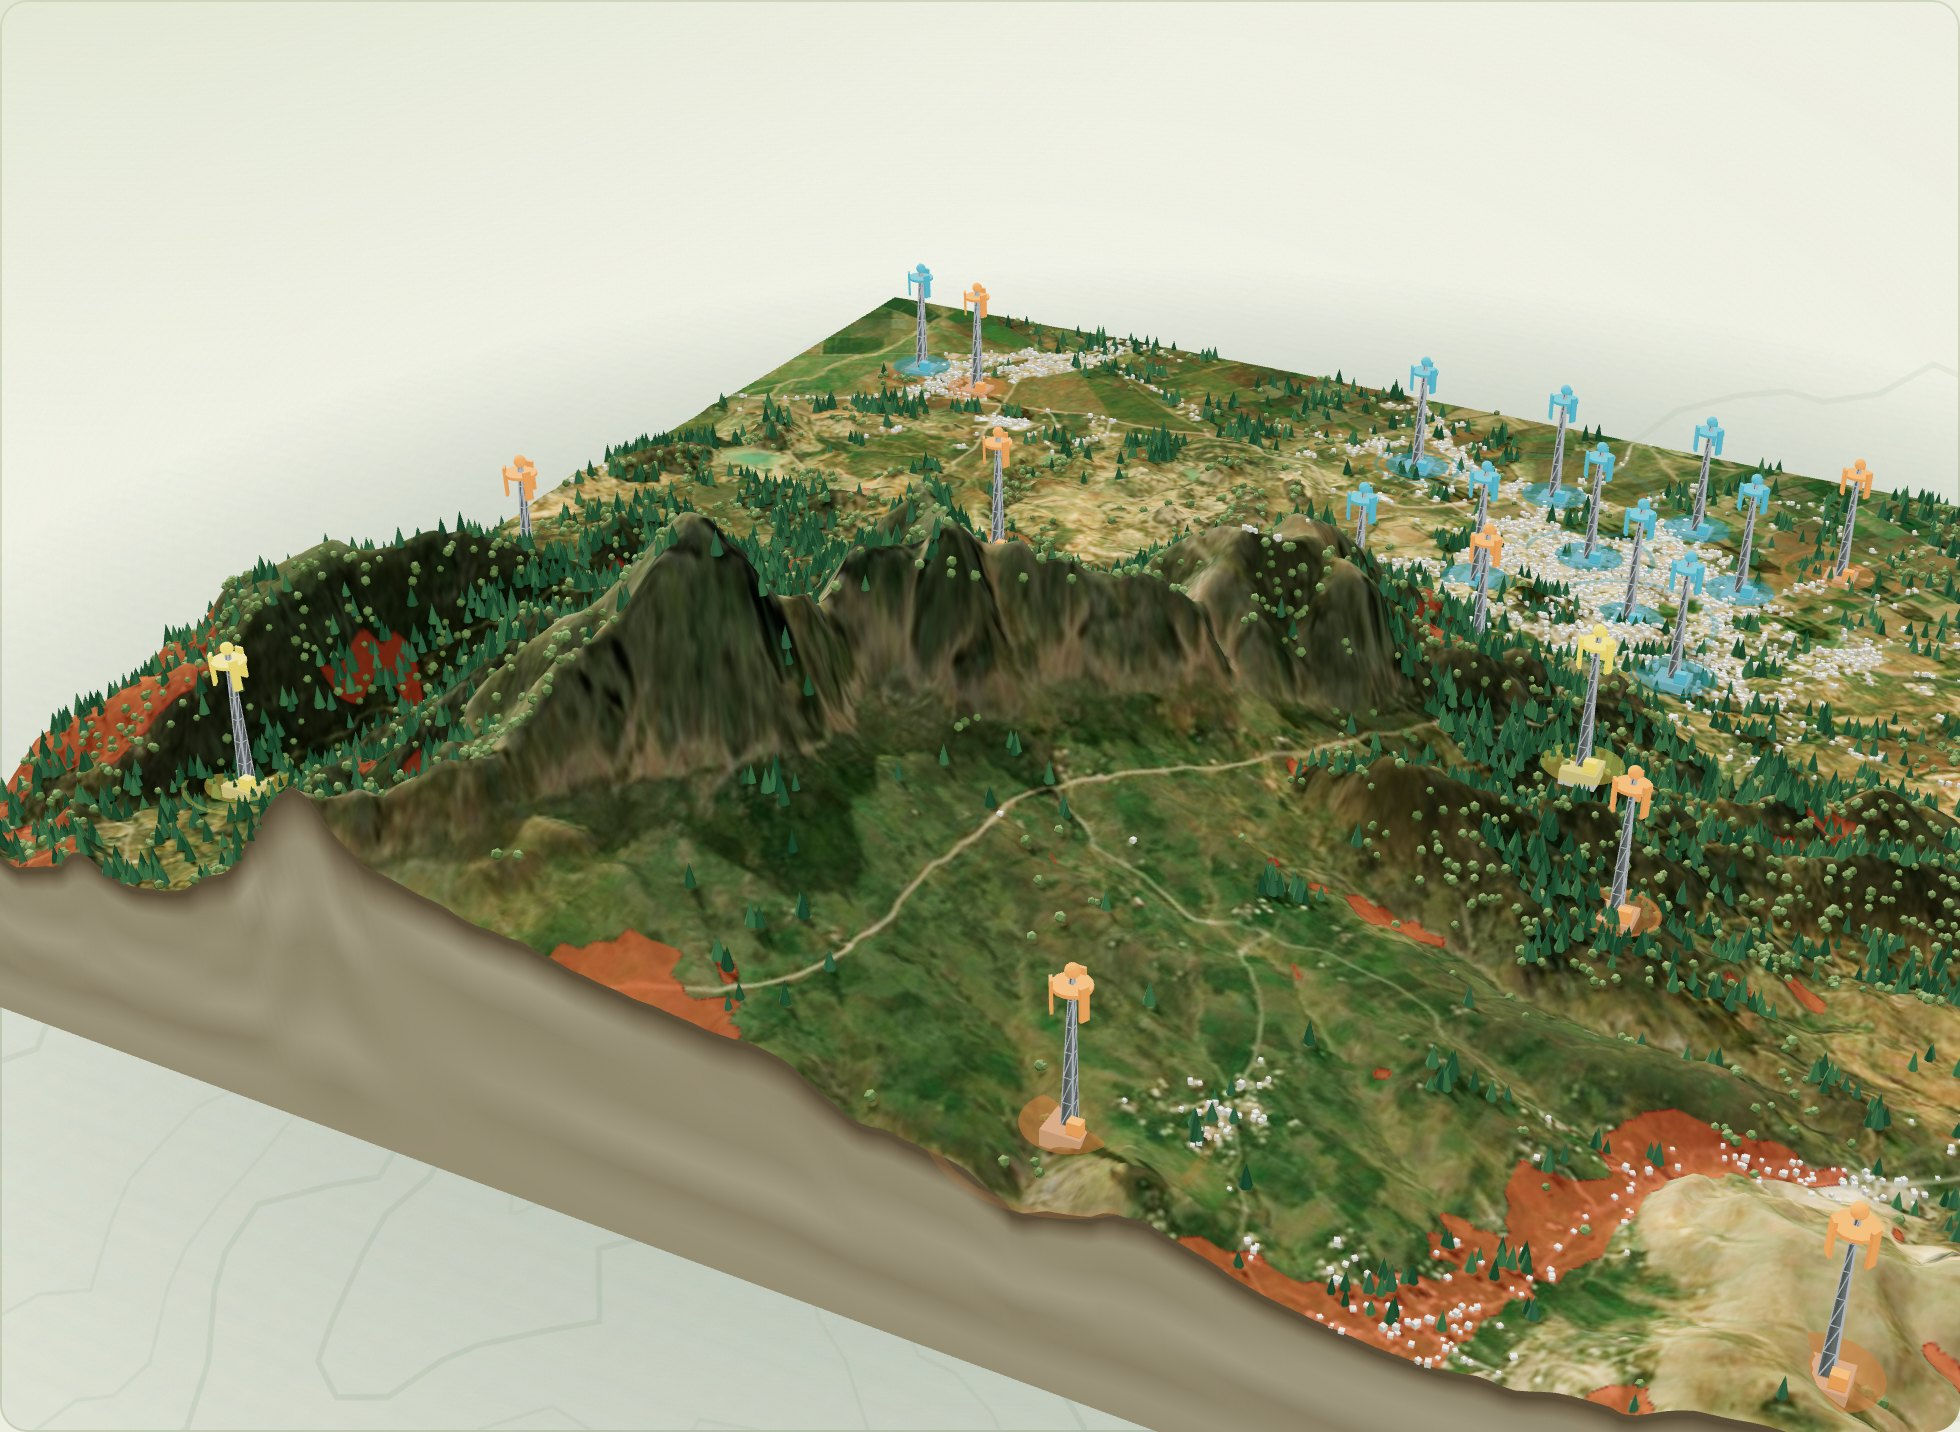
\includegraphics[width=0.62\textwidth]{ombre-final.jpg}
\caption{Le réseau final sur le relief.}
\label{fig-ombre-final}
\end{figure}

\begin{table}[H]
\centering
\caption{Réseau initial et réseau final.}
\label{tab-final}
\begin{tabularx}{\textwidth}{@{}Lccc@{}}
\toprule
\thead{Indicateur} & \thead{Initial} & \thead{Final} & \thead{Objectif} \\
\midrule
Couverture urbaine indoor & \SI{99,5}{\percent} & \textbf{\SI{99,7}{\percent}} & \SI{95}{\percent} \ok \\
Couverture rurale (surface / population) & \SI{83,4}{\percent} / \SI{95,4}{\percent} & \textbf{\SI{94,3}{\percent}} / \SI{97,9}{\percent} & \SI{95}{\percent} ($-0{,}7$ pt) \\
DL $\geq \SI{1}{\Mbps}$, ville (surface / population) & \SI{78,9}{\percent} / \SI{77,4}{\percent} & \SI{79,4}{\percent} / \SI{77,7}{\percent} & \SI{95}{\percent} \ko \\
DL $\geq \SI{1}{\Mbps}$, campagne (surface / population) & \SI{38,0}{\percent} / \SI{58,9}{\percent} & \SI{54,5}{\percent} / \SI{67,9}{\percent} & \\
UL $\geq \SI{128}{\kbps}$, ville & \SI{99,5}{\percent} & \SI{99,7}{\percent} & \SI{95}{\percent} \ok \\
UL $\geq \SI{128}{\kbps}$, campagne (surface / population) & \SI{55,8}{\percent} / \SI{83,0}{\percent} & \SI{73,9}{\percent} / \SI{89,6}{\percent} & \\
Surface couverte (toute la carte) & \SI{73,8}{\kilo\metre\squared} & \SI{86,8}{\kilo\metre\squared} & \\
Surface à 4 serveurs ou plus & \SI{2,39}{\kilo\metre\squared} & \SI{0,91}{\kilo\metre\squared} & \\
Nombre de sites & 20 & 21 & 21 (Étape 1) \\
\bottomrule
\end{tabularx}
\end{table}

Le \cref{tab-final} utilise les prédictions outdoor sauf mention, avec les charges simulées à \num{1000} utilisateurs. Pour les lignes DL et UL, la colonne \enquote{initial} est le réseau après l'action 1, recalculé avec les charges simulées (\cref{sec-charge}).

\subsection{Le Monte-Carlo final}

\begin{table}[H]
\centering
\caption{Monte-Carlo à \num{1000} utilisateurs, avant et après.}
\label{tab-mc-final}
\begin{tabular}{@{}lccc@{}}
\toprule
\thead{Indicateur} & \thead{Réseau initial} & \thead{Réseau final} & \thead{Évolution} \\
\midrule
Utilisateurs rejetés & 108,3 (\SI{10,8}{\percent}) & \textbf{76,8 (\SI{7,7}{\percent})} & $-\SI{29}{\percent}$ \\
\quad pas de couverture & 26,6 & 12,85 & divisé par 2 \\
\quad pas de service & 81,7 & 63,95 & $-\SI{22}{\percent}$ \\
\quad saturation & 0 & 0 & \\
Débit DL servi (cumulé) & \SI{257,3}{\Mbps} & \SI{281,1}{\Mbps} & $+\SI{9}{\percent}$ \\
Débit UL servi (cumulé) & \SI{68,3}{\Mbps} & \SI{70,5}{\Mbps} & $+\SI{3}{\percent}$ \\
\bottomrule
\end{tabular}
\end{table}

\begin{figure}[H]
\centering
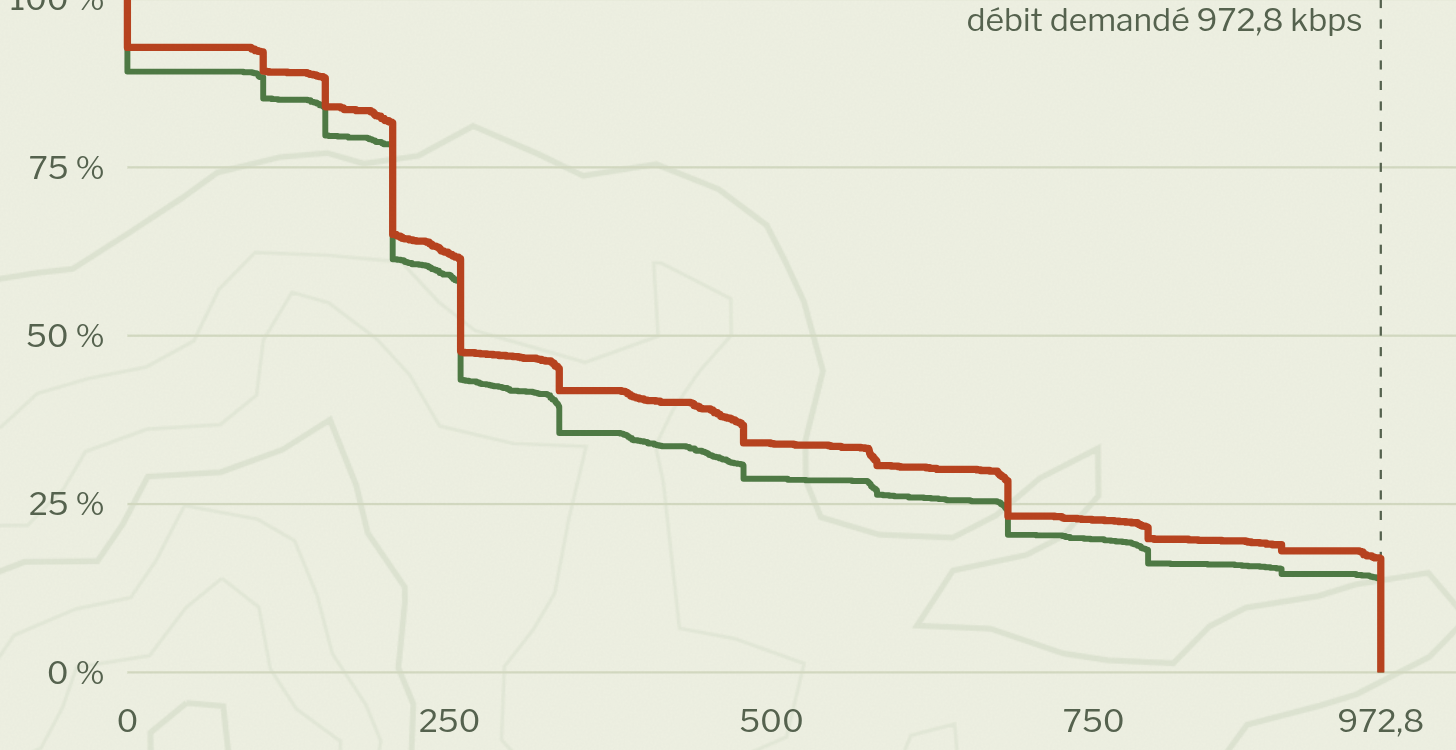
\includegraphics[width=0.66\textwidth]{dcfi-avant-apres.png}
\caption{DCFI DL à \num{1000} utilisateurs, avant et après.}
\label{fig-dcfi-final}
\end{figure}

Le \cref{tab-mc-final} donne la moyenne des 20 tirages, avec la même graine. Sur la \cref{fig-dcfi-final} (utilisateurs HSI, réseau initial en vert, final en terre cuite), toute la courbe monte d'environ 4 points : sur l'échantillon tracé, les rejets passent de \SI{10,5}{\percent} à \SI{6,7}{\percent} et la part des utilisateurs HSI servis au débit demandé de \SI{13,8}{\percent} à \SI{16,8}{\percent}. La médiane reste à \SI{259}{\kbps} : à \num{1000} utilisateurs, la limite est la capacité, que l'optimisation de la couverture ne règle pas (\cref{sec-p4}).

\subsection{Les mêmes utilisateurs, avant et après}

La graine fixée permet une comparaison directe : Atoll tire exactement les mêmes \num{1041} utilisateurs (mêmes positions, mêmes services) sur les deux réseaux. On peut donc suivre chaque utilisateur (\cref{fig-memes}). Sur la carte, un anneau or marque un utilisateur rejeté au départ et connecté sur le réseau final, un cercle creux terre cuite un utilisateur connecté au départ puis perdu, et une croix un utilisateur toujours rejeté.

\begin{figure}[H]
\centering
\begin{subfigure}[b]{0.5\textwidth}\centering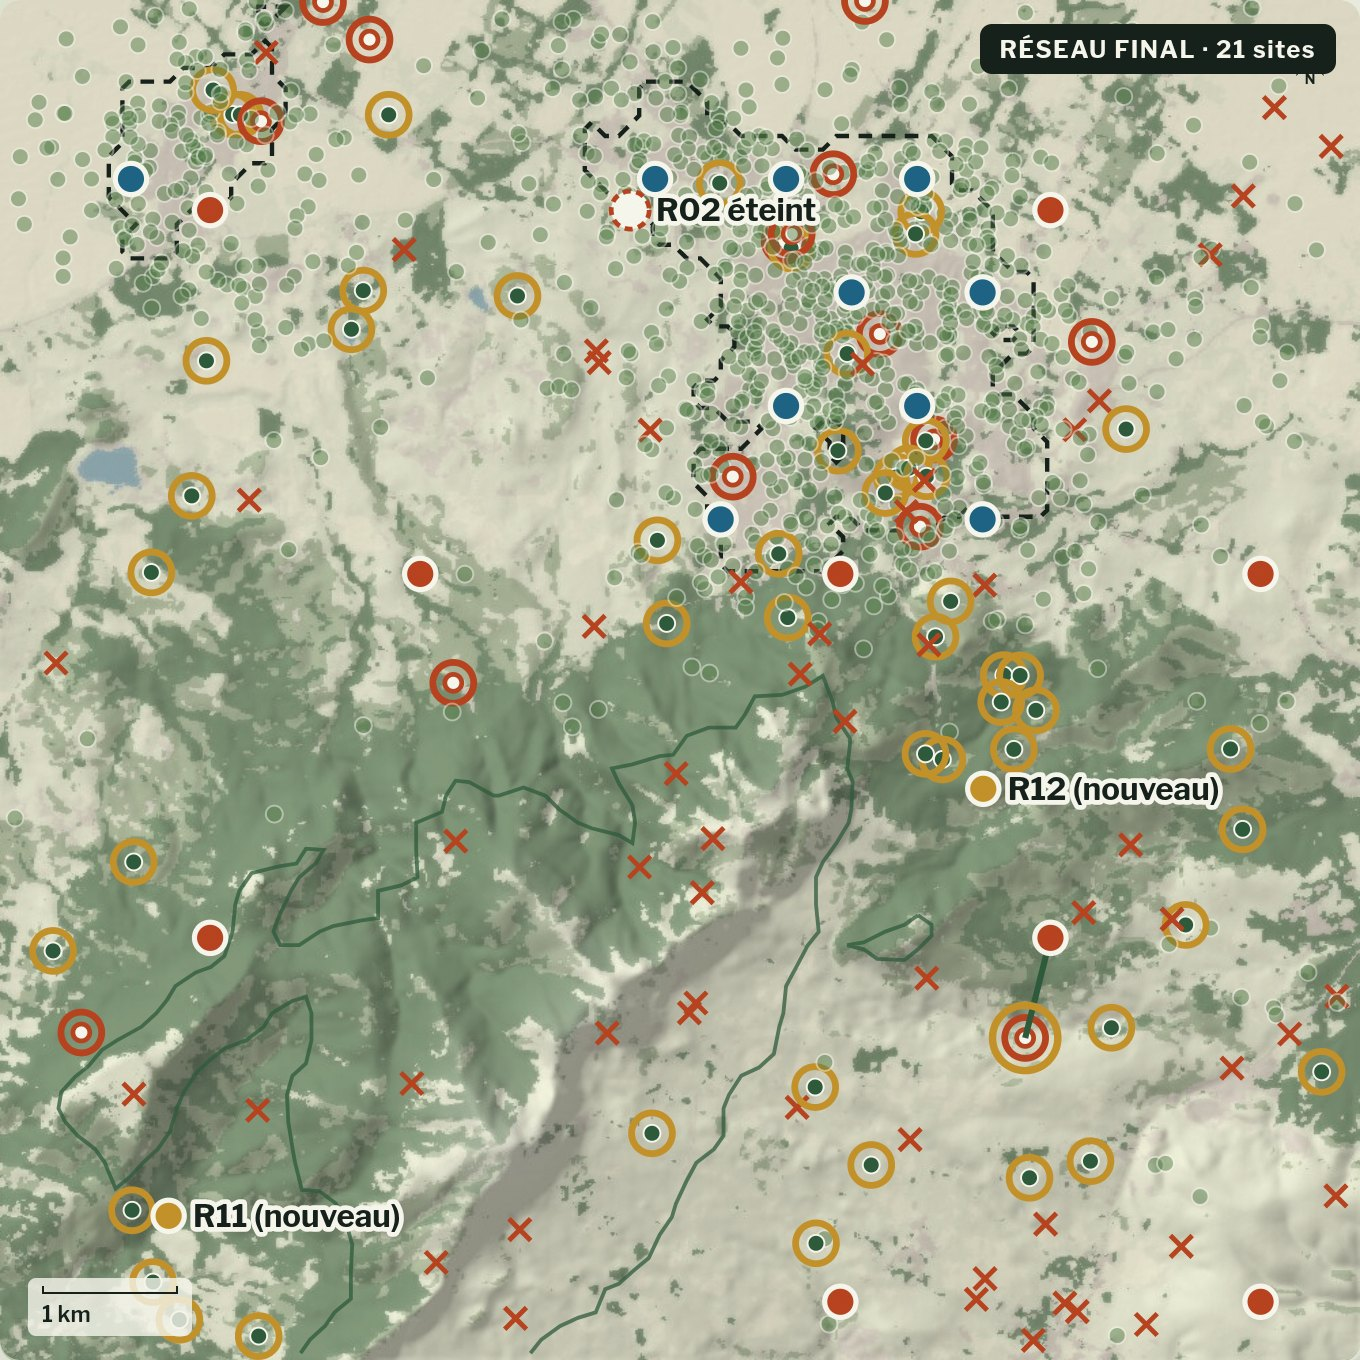
\includegraphics[width=\textwidth]{memes-utilisateurs.jpg}\caption{Réseau final.}\end{subfigure}\hfill
\begin{subfigure}[b]{0.47\textwidth}\centering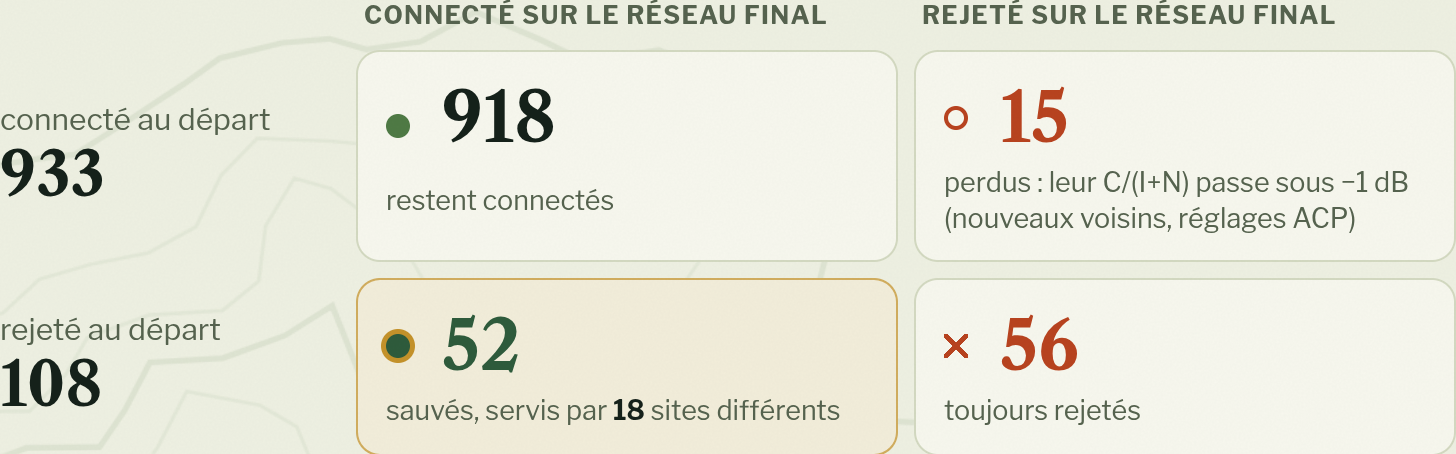
\includegraphics[width=\textwidth]{matrice-transitions.png}\caption{Transitions.}\end{subfigure}
\caption{Les mêmes \num{1041} utilisateurs sur les deux réseaux.}
\label{fig-memes}
\end{figure}

\begin{itemize}
  \item 52 utilisateurs rejetés sont sauvés. Ils sont servis par 18 sites différents, donc le gain vient de l'ensemble des actions (R11, R12 et les réglages de l'ACP). Par exemple, un utilisateur du coin sud-ouest sans couverture sur le réseau initial est servi par R11 avec un C/(I+N) de \SI{17,1}{\deci\bel}.
  \item 15 utilisateurs connectés sont perdus : leur C/(I+N) passe sous \SI{-1}{\deci\bel}, car les nouveaux sites et les réglages de l'ACP déplacent l'interférence.
  \item Au total, les rejetés passent de 108 à 71. Les 71 restants se trouvent dans la campagne isolée (46), sur le massif sans objectif (13) et en ville (12, dont 11 à l'intérieur des bâtiments), où la cause est l'interférence entre sites urbains.
\end{itemize}

\begin{retenir}
Cinq actions gardées (tilt urbain, R02 désactivé, R11, R12, ACP), trois rejetées après mesure (R07 déplacé, R07 réorienté, tilt à \ang{8}) et les relations de voisinage (ANR). La couverture rurale passe de \SI{83,4}{\percent} à \SI{94,3}{\percent}, la couverture urbaine reste au-dessus de \SI{99}{\percent}, avec 21 sites, et les rejets à \num{1000} utilisateurs passent de \SI{10,8}{\percent} à \SI{7,7}{\percent}.
\end{retenir}
